\usetikzlibrary{calc}
\usetikzlibrary{arrows.meta}

\tikzset{
    base above/.style={anchor=base, yshift=\pgfkeysvalueof{/pgf/inner ysep}},   % for "m" VS "p" vertical alignment of labels
    start/.style={very near start,base above,sloped},
    end/.style={very near end,base above,sloped}
    }

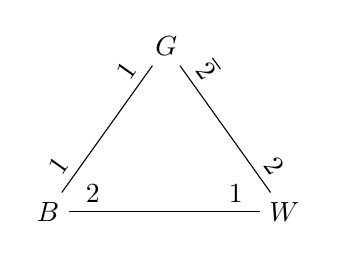
\begin{tikzpicture}
	\def\scale{3}
	\node (B) at (0,0) {$B$};
	\node (W) at (1*\scale,0) {$W$};
	\node (G) at (0.5*\scale,0.7*\scale) {$G$};

	\draw (B)--(G)
		node[start] {$1$}
		node[end] {$1$};
	\draw (B)--(W)
		node[start] {$2$}
		node[end] {$1$};
	\draw (W)--(G)
		node[start] {$2$}
		node[end] {$\overline 2$};
\end{tikzpicture}